\chapter{Software de adquisición}
\label{cap2}
En este capítulo procederemos a explicar el funcionamiento del software de adquisición. Empezaremos recordando los aspectos básicos descritos en el
capítulo \ref{cap1}. El software de adquisición es el encargado de coordinar la estación. El funcionamiento nominal del software consiste en recoger
la información de los demás módulos y guardar la en una base de datos. Aparte de dotarle de esta funcionalidad nominal el software debe ser capaz de
iniciarse automáticamente y recuperarse ante posibles fallos.  
\par
El software se ejecuta sobre un Linux en una placa BeagleBone Black\cite{Beagle}\cite{BeagleWiki}. El lenguaje utilizado para el desarrollo del
software es Python\cite{Python}. Para la gestión de la base de datos hemos elegido Sqlite3\cite{Sqlite}. Al ser un software para un sistema empotrado
es conveniente estar familiarizados con el entorno hardware, descrito en el capítulo \ref{entornoHW}.
\par
En la figura \ref{fig:soft_adquisición} podemos ver un diagrama de flujo que describe el funcionamiento de nuestro software. A lo largo de este
capítulo haremos muchas referencias a este diagrama para explicar los diferentes módulos software que lo componen. Podemos ver que hay 4 módulos
principales, a continuación haremos una breve descripción de estos. 

\begin{itemize}
  	\item	\texttt{NMDA}. Es el proceso principal de nuestro software. Este es el encargado de realizar las configuraciones necesarias e iniciar
	  	el \texttt{FPGASerialReader} y el \texttt{CountsManager}.
	\item	\texttt{FPGASerialReader}. Thread que se encarga de procesar la información transmitida por la FPGA.
	\item	\texttt{CountsManager}. Thread que se encarga de pedir la información necesaria y guardarla en la base de datos con periodicidad de un
	  	minuto. Después de guardar la información de un nuevo minuto este inicia el \texttt{DBUpdater}.
	\item	\texttt{DBUpdater}. Thread que se encarga de sincronizar la base de datos local con la replica remota.
\end{itemize}

\begin{sidewaysfigure}[p]
	\centering
	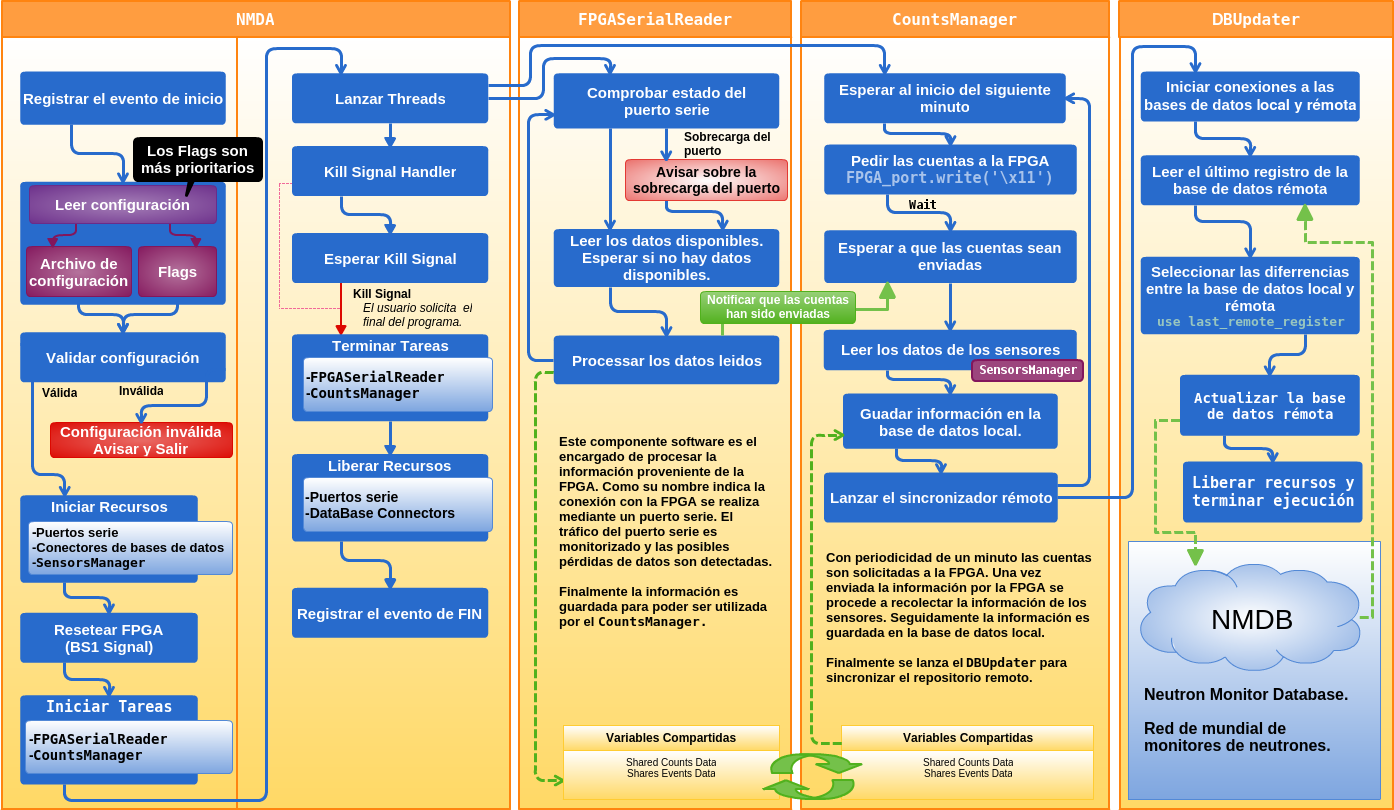
\includegraphics[keepaspectratio, width=1\textwidth]{./img/soft_adquisicion.png}
	\caption{Diagrama de flujo. Software de adquisición.}
	\label{fig:soft_adquisición}
\end{sidewaysfigure}

\section{Arranque automático del sistema}
	Uno de los requisitos del sistema es que se ponga en marcha automáticamente ante la presencia de corriente eléctrica. La BeagleBone Black por
	defecto está configurada para que arranque automáticamente. Nos queda configurar el sistema operativo para que arranque nuestro software de
	forma automática. Para este propósito vamos a utilizar las \emph{System Services}\cite{AngSystemctl} que Angstrom nos ofrece. No vamos a
	explicar muy a fondo el funcionamiento de estas, están muy bien explicadas en la bibliografía citada. Tan solo nos interesa resaltar que nos
	permiten arrancar nuestro software de forma automática.
	\par
	En la figura \ref{fig:boot} podemos ver la secuencia de arranque del sistema. Vemos que antes de arrancar el software de adquisición tenemos
	que realizar una serie de tareas. En los puntos siguientes describiremos estas tareas.
	\begin{figure}[h]
		\centering
		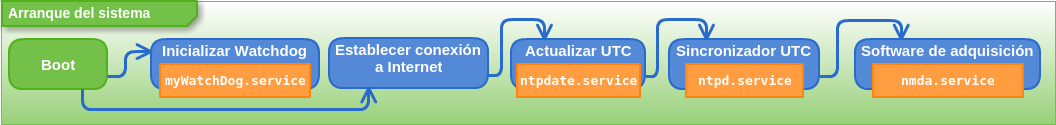
\includegraphics[keepaspectratio, width=1\textwidth]{./img/boot.png}
		\caption{Arranque del sistema}   %TODO monospace
		\label{fig:boot}
	\end{figure}
	\subsection{Watchdog}
		Un Watchdog \cite{WatchDogWiki} es un mecanismo de seguridad que realizar un Reset en el sistema cuando se detecta un
		malfuncionamiento. Consiste en un temporizador que realiza una cuenta atrás, cuando esta cuenta llega a cero el sistema es reiniciado.
		Es nuestro software el que debe reiniciar este contador para que no expire. Los Watchdogs pueden ser software o hardware, el que
		utilizamos nosotros esta implementado en la BeagleBone Black y es hardware.
		\par
		El código que activa y resetea el Watchdog está en el archivo \texttt{WatchDog.py}. Consite en un proceso que periódicamente reinicia
		el timer. Actualmente no tiene gran funcionalidad mas que asegurarse de que el sistema operativo sigue funcionando. Si el sistema
		operativo se queda bloqueado el timer no será reiniciado, por lo que el Watchdog procederá a reiniciar todo el sistema. A continuación
		podemos ver el código fuente del \texttt{Watchdog.py}.
		\begin{lstlisting}
import time
import os
# Damos gran prioridad a este proceso
os.nice(20)
# Abriendo el siguiente archivo ponemos en marcha el Watchdog hardware
wd = open(''/dev/watchdog'', ''w+'')
while 1:
	# Escribiendo en el archivo reiniciamos el timer del Watchdog
	wd.write(''\n'')
	wd.flush() 
	time.sleep(20)
		\end{lstlisting}
		Actualmente estamos planteándonos realizar una versión más avanzada del Watchdog, sobre esto hablaremos más a fondo en el capítulo 
		\ref{cap_conclusiones}.
	\subsection{Sincronización UTC}
		La BeagleBone Black no implementa ningún mecanismo hardware para calcular la fecha y hora actuales, por lo que en cada reinicio la
		fecha y hora se pierden. Es nuestra responsabilidad realizar un mecanismo software que nos sincronice con el resto del mundo\cite{ntpd}.
		Utilizaremos el programa \texttt{ntpd} para este propósito. \texttt{ntpd} es un programa que hace uso del 
		\emph{Network Time Protocol}\cite{ntpWiki} para mantener el tiempo del sistema. Haremos dos llamadas a este programa.
		\begin{lstlisting}
# Actualiza la fecha y hora.
/usr/bin/ntpd -q -g -x
# Lanza un demonio que corrige las derivas que puedan presentarse
/usr/bin/ntpd -p /run/ntpd.pid
		\end{lstlisting}


\section{\texttt{NMDA}}
	Este es el módulo principal de nuestro software. En la figura \ref{fig:soft_adquisición} podemos ver un diagrama de flujo que representa el
	funcionamiento de este. En las siguientes subsecciones describiremos las funcionalidades más relevantes de este módulo.
	\subsection{Logger}
		Haciendo uso de la librería \texttt{logging}\cite{py_logging} configuramos un archivo de Log. En este archivo iremos registrando eventos importantes
		que sucedan. Ejemplo de eventos que registramos son las pérdidas de datos o el inicio del sistema. El mecanismo está configurado para
		que automáticamente se guarde la hora y fecha de cada mensaje. A continuación se muestra como se configura y usa este mecanismo.
		\begin{lstlisting}
import logging
logging.basicConfig(filename='/server/logs/NMDA.log', level=logging.DEBUG, format=''%(asctime)s   %(message)s'')
logging.info('Started')
		\end{lstlisting}
	\subsection{Archivo de configuración y Flags}
		Existen una serie de variables que varían en función de la estación o que simplemente pueden cambiar con el tiempo. No es buena idea
		tener los valores de estas variables en el código. Este problema nos ha llevado a exportar estas variables a un archivo de configuración.
		Para leer este archivo utilizamos la librería \texttt{ConfigParser}\cite{py_ConfigParser}. A continuación mostramos un ejemplo de este
		archivo que nos ayudara a entender mejor su estructura.
		\begin{lstlisting}
[Basics]
# The serial RS232_FPGA1C
serial_port_control  = /dev/ttyO2
# The local database where data will be saved. If 'shell' is specified as database data will be printed to the shell
database = /server/data/test.db

[Sensors]
# The serial RS232_FPGA1
serial_port_sensors= None
# The type of barometer that will be used. 'None', 'bm35', 'ap1'
barometer_type = None
# The type of hvps that will be used. 'None', 'analog', 'digital'
hvps_type = None
#Correction coefficient for the analog hvps, 1.0 ==> No correction
analog_hvps_corr = 1.0

[dbUpdater]
db_updater_enabled=True
# Must be the same that Basic.database
local_db= /server/data/test.db 
# The remote database config
remote_db_host= 192.168.1.1
# The user must have privileges
remote_db_user= hristo
remote_db_pass= 123qwe
# The database will be created if not exists along with all the tables
remote_db_db= nmdadb2
		\end{lstlisting}
		Los valores de las variables exportadas son también accesibles mediante el uso de Flags. En este caso hemos utilizado la librería 
		\texttt{argparse}\cite{py_argparse}. Los valores que son especificados con Flags sobrescriben a los valores del archivo de
		configuración. Los Flags se usan de la siguiente forma.
		\begin{lstlisting}
#TODO TODO TODO  Arrancar el programa con el flag -h y copiar lo que imprima 
		\end{lstlisting}
	\subsection{Iniciar recursos}
		Al ser el módulo principal, \texttt{NMDA} es el encargado de iniciar todos los recursos que serán utilizados. Por recursos nos
		referimos a las variables compartidas, conectores a las bases de datos, interfaces de los puertos serie y otros. Lo más interesante de
		este apartado es que las tablas de las bases de datos son creadas automáticamente si no existen. Esto simplifica mucho la tarea de
		implantar el software.
	\subsection{Resetear FPGA}
		Como hemos explicado en el capítulo \ref{entornoHW} la FPGA nos permite realizar un Reset, nuestro software realizara uno antes de
		empezar con la adquisición de datos. Este Reset nos asegura que la FPGA estará en un correcto estado. Para realizar el Reset de la
		FPGA utilizaremos la entrada digital que está conectada al pin \emph{P9\_42} de la BeagleBone Black. Volvemos a recordar que la señal
		digital es activa a nivel bajo. Para controlarla utilizaremos la librería de \emph{AdaFruit}\cite{AdaFruitGit} de la siguiente manera.
		\begin{lstlisting}
import Adafruit_BBIO.GPIO as GPIO
GPIO.setup('P9_42', GPIO.OUT)
GPIO.output('P9_42', GPIO.LOW)
time.sleep(0.5)
GPIO.output('P9_42', GPIO.HIGH)
		\end{lstlisting}
	\subsection{Iniciar Tareas}
		El siguiente paso es iniciar los dos Threads, \texttt{CountsManager} y \texttt{FPGASerialReader}. Son estos dos Threads los que
		realizan todo el proceso de adquisición, serán descritos más adelante en este capítulo. 
	\subsection{Kill Signal Handler}
		Este es un software que debe ejecutarse indefinidamente. En su uso real no será interrumpido, pero hemos implementado un mecanismo que
		nos permite pararlo. Este mecanismo nos permite solicitar el fin del programa, que desencadena una serie de acciones. Estas acciones
		tienen como objetivo asegurar que todos los recursos sean liberados de forma correcta. Liberar los recursos de forma correcta supone
		no tener ningún problema si seguidamente volvemos a ejecutar el software. Esto en el uso real del software no tiene gran impacto, sin
		embargo ha sido muy útil en el proceso de desarrollo.

\section{\texttt{FPGASerialReader}}
	Este módulo software es el encargado de leer y procesar los datos transmitidos por la FPGA. En la figura \ref{fig:soft_adquisición} podemos
	ver un diagrama de flujo que refleja el funcionamiento de este. La ejecución del Thread empieza comprobando el estado del puerto serie, que
	puede estar saturándose. En el caso de que el puerto se esté saturando es generada una estrada en el archivo de Log. A continuación leemos
	los datos disponibles, en caso de no haber datos disponibles el Thread se queda bloqueado esperando a la llegada de estos. Seguidamente de
	leer los datos pasamos a procesar los, por procesar nos referimos a interpretar el significado que tienen. Finalmente volvemos al paso inicial.  
	\par
	En las tablas del capítulo \ref{entornoHW} podemos ver el formato de los datos que tenemos que procesar. Vemos que hay tres tipos de mensajes
	que podemos recibir. Los mensajes no siguen un orden concreto, además llegan de forma totalmente asíncrona. Los mensajes son transmitidos en
	forma de bytes. El canal de transmisión no asegura la correcta transmisión de los bytes por lo que algunos se pueden perder. Todo esto
	conlleva a que procesar los datos no sea tarea fácil.
	\par
	Para este propósito hemos implementado una máquina de Moore. Si nos volvemos a fijar en el formato de los datos podemos ver que los primeros
	bits de cada byte son fijos. Estos bits nos ayudan a identificar a que mensaje corresponde el byte. Los estados y transiciones de la maquina
	pueden verse en la figura \ref{fig:reader}. El estado inicial es \texttt{ByteX}. Aunque no esté reflejado en la figura la recepción de cualquier
	valor no esperado nos lleva al estado inicial.
	\par
	La información generada al procesar los datos es almacenada en las variables compartidas. Estas variables son accesibles desde el 
	\texttt{CountsManager}.
	\begin{figure}[h]
		\centering
		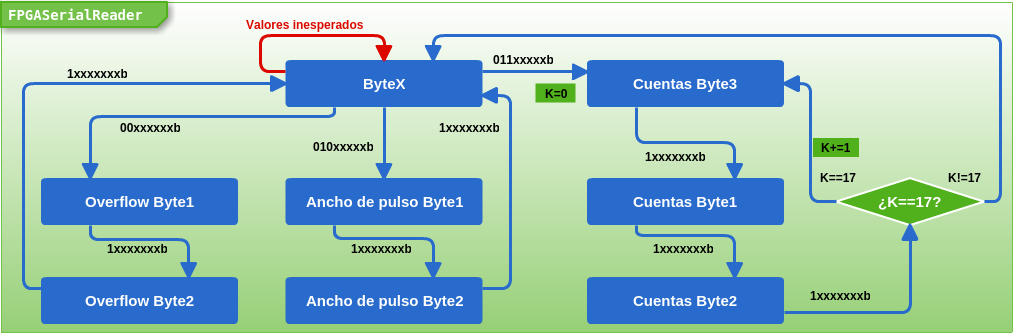
\includegraphics[keepaspectratio, width=1\textwidth]{./img/reader.png}
		\caption{Máquina de Moore. \texttt{FPGASerialReader}.}   %TODO monospace
		\label{fig:reader}
	\end{figure}

\section{\texttt{CountsManager}}
	Intro funcionamineto.
	\subsection{Deriva local}
	\subsection{Petición de cuentas}
	\subsection{Petición de datos sensores}
	\subsection{Guardar datos}
\section{\texttt{DBUpdater}}
	Este módulo software es el encargado de actualizar el contenido de la base de datos remota. El funcionamiento de este es muy simple y se puede
	ver en la figura \ref{fig:soft_adquisición}. Empieza estableciendo la conexión con la base de datos remota. Si esta se establece procede a leer la
	última entrada en la base de datos remota. Seguidamente el software calcula la diferencia entre las dos bases de datos, para el propósito usa
	la fecha y hora de la entrada leída de la base de datos remota. Finalmente el software selecciona las diferencias entre las dos bases de datos
	y las escribe en la remota. Es entonces cuando la ejecución de este Thread termina. 
	\par
	Si la conexión con la máquina que alberga a la base de datos remota se pierde por un tiempo, cuando esta vuelva a restablecerse el 
	\texttt{DBUpdater} sincronizara las dos bases de datos. Eventualmente si las diferencias entre las dos bases de datos son muy grandes la
	sincronización no ocurrirá de golpe, de esta manera evitamos sobrecargar al sistema. El fallo de la sincronización no es crítico, el Thread
	volverá a ser lanzado el próximo minuto y volverá intentar sincronizar las dos bases de datos.


\section{\texttt{SensorsManager}}
	\subsection{Pressure}
	\subsection{HVPS}

\section{testing}
	Porque son importantes los unit tests.
	\subsection{moking}
	\subsection{Coverage}

\section{Mantenimiento}
	Dejar el sistema de adquisición de datos funciónando algun tiempo. Hacer analisis de los datos. Describir experiencia.  TODO dejar para el capítuo de Conclusiones.
